% Assignment 1 report template. At most three pages.
% Fill in every section; keep the headings. Compile with pdflatex.
\documentclass[11pt,a4paper]{article}
\usepackage[margin=2.2cm]{geometry}
\usepackage{graphicx,booktabs,amsmath,hyperref,listings}
\title{Assignment 1: Train a minimal language model from scratch}
\author{Samina Kadkhoda Masoumali (52308861, Informatik)}
\date{\today}
\usepackage{float}
\usepackage{booktabs}
\begin{document}
\maketitle

\section{Tokenizer (R1)}
% training time, peak memory, longest token, the first twenty merges, bytes/token on the
\begin{itemize}
\item \textbf{Training on tinystories train}
    \begin{itemize}
    \item Peak memory: 89767936 bytes
    \item Training time: 1251.0382787999697 secs (20.850637979999494 mins)
    \item Longest token: b' accomplishment' (length: 15 bytes)
    \item First 20 merges: [(b' ', b't'), (b'h', b'e'), (b' ', b'a'), (b' ', b's'), (b' ', b'w'), (b'n', b'd'), (b' t', b'he'), (b'e', b'd'), (b' ', b'b'), (b' t', b'o'), (b' a', b'nd'), (b' ', b'h'), (b' ', b'f'), (b'i', b'n'), (b' ', b'T'), (b' w', b'a'), (b'r', b'e'), (b'i', b't'), (b'o', b'u'), (b' ', b'l')]
    \end{itemize}
    
% TinyStories validation text and on the OpenWebText sample, encoding throughput.
\item \textbf{Evaluating on tinystories valid}
    \begin{itemize}
    \item Tokenization time: 82.96440749999601 secs
    \item Throughput: 0.27123198583683106 MB/s
    \item Bytes per token: 4.116920379913068
    \end{itemize}
\item \textbf{Evaluating on owt valid}
    \begin{itemize}
    \item Tokenization time: 1198.1350417999784 secs
    \item Throughput: 0.24204179235449957 MB/s
    \item Bytes per token: 3.173861047131087
    \end{itemize}
\end{itemize}

% Two sentences: what does the bytes-per-token difference tell you?
On the tinystories text, the model could fit more bytes into one token, compared to the owt text, which means for processing the same bytes of text in both samples, we would need less tokens in tinystories. Also if we have a limit for the total tokens available, we can process more text in tinystories compared to owt. So tinystories text is better for compression.


\section{Sanity checks (R2)}
% initial loss, the overfit-one-batch curve (figure), the resume test.
\begin{itemize}
\item Initial loss: 9.270365715026855
\item The resume test: the run resumed from step 101 and finished
\item The overfit-one-batch curve:
\begin{figure}[H]
    \centering
    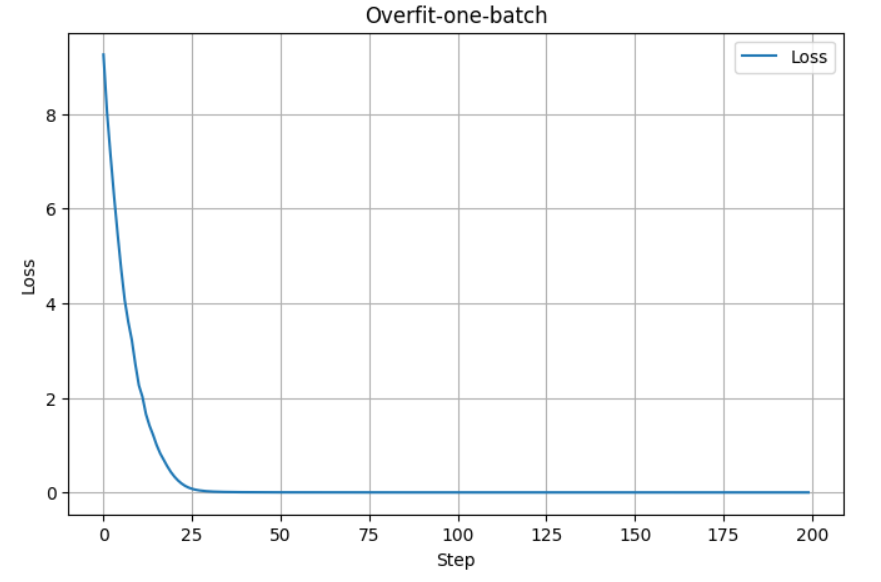
\includegraphics[width=0.5\linewidth]{overfit.png}
    \caption{Training loss recorded repeatedly while training on one fixed batch. The loss comes below 0.1 at step 23.}
    \label{fig:overfit}
\end{figure}  
\end{itemize}



\section{Learning-rate sweep (R3)}
% figure: final validation loss vs learning rate (log axis); the chosen rate.
\begin{figure}[H]
    \centering
    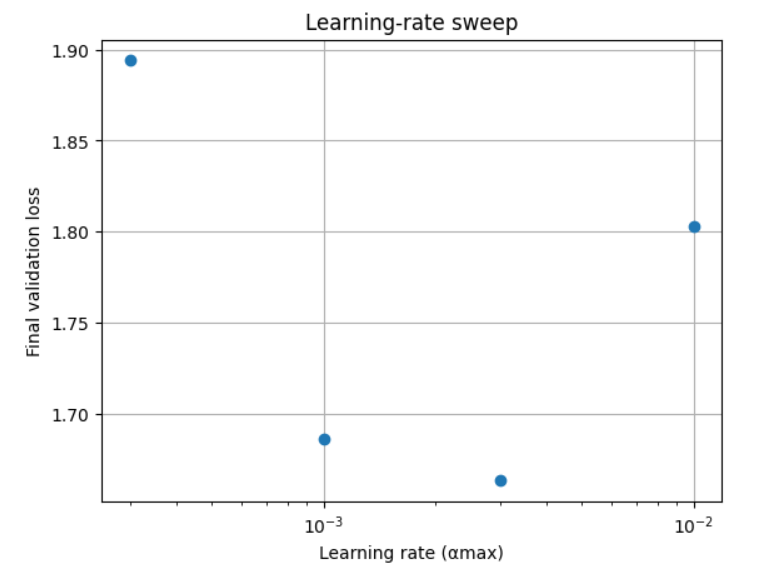
\includegraphics[width=0.5\linewidth]{sweep.png}
    \caption{Final validation loss in runs with learning rates 0.0003, 0.001, 0.003, 0.01. The best rate is 0.003 with the lowest loss 1.663.}
    \label{fig:sweep}
\end{figure}

\section{Reference run (R4)}
% figure: train and validation loss (log-scale x). Final validation loss, GPU, tokens/s, MFU.
\begin{itemize}
\item{Final validation loss: 1.4422505274415016}
\item{GPU: Tesla T4}
\item{Tokens/s: 27362.148836421435}
\item{MFU: 0.047030270214284596}
\end{itemize}
\begin{figure}[H]
    \centering
    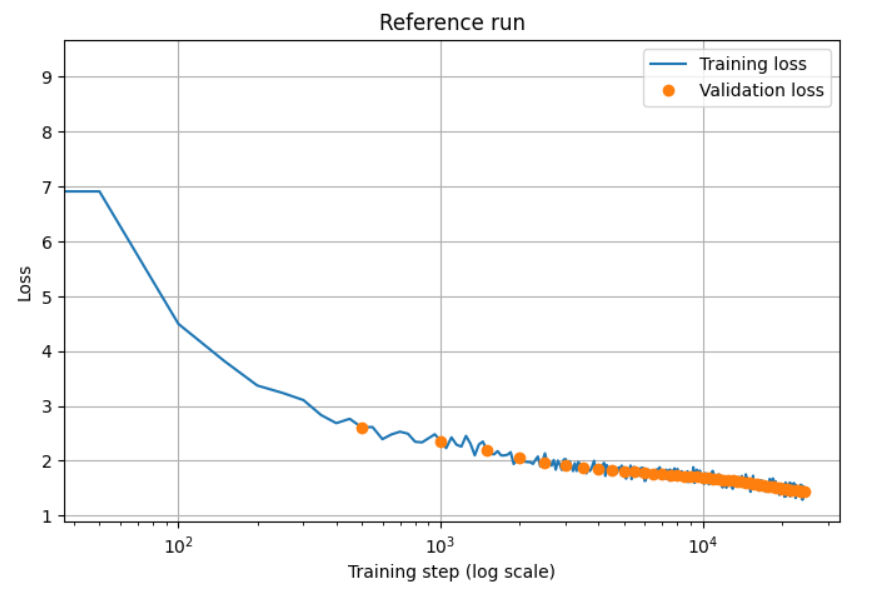
\includegraphics[width=0.5\linewidth]{ref_step_loss.png}
    \caption{Training and validation loss retrieved from json log files after reference run. The loss in both samples are decreasing over the steps.}
    \label{fig:ref_step_loss}
\end{figure}

\section{Efficiency table (R5)}
\begin{table}[h]\centering
\begin{tabular}{@{}lrr@{}}\toprule
Configuration & tokens/s & MFU \\\midrule
eager fp32 & 17665.10116038851 & 0.030356796917159947\\
+ autocast & 33317.15464290594 & 0.057254248824809124\\
+ \texttt{F.scaled\_dot\_product\_attention} & 54434.21741950837 & 0.09354310901167823\\
+ fused \texttt{AdamW} & 58578.47984669711 & 0.10066486459809335\\
+ \texttt{torch.compile} & 85241.8108361401 & 0.14648477339072077\\\bottomrule
\end{tabular}
\end{table}
% one paragraph: which change moved which bar of your profile?
I used the profiler for each run in each case and traced 5 steps. The change from eager to autocast, reduced total time from 2.401s to 1.245s, which is almost cut by half. Also aten::bmm time is reduced significantly, falling from 1.362s to 196.914ms. \newline
After using torch sdpa instead of my own implementation,total time becomes 752ms and total time of aten::copy was reduced from 201.280ms to 99.134ms. Other attention operations such bmm and mul have dropped as well. \newline
Replacing my AdamW implemantation with torch.optim.adamw, reduces the total time to 702ms and the number of aten::mul calls drop to 715, which used to be about 1800 in the previous versions. Also the Optimizer.step#AdamW.step is no longer among the top 20, which means its runtime is reduced. \newline
By using torch.compile, the total time is dropped to 479ms, and most of the top 20 contains compile-related features.


\section{Ablation (R6)}
% name, prediction (written before the run), measurement, explanation.
\begin{itemize}
\item{Choosen case: no warmup}
\item{Predicted loss(before the run): 1.75}
\item{Calculated loss: 1.7535251043736935}
\end{itemize}
In 4883 steps and fraction of 0.05 for warmup, we use the first 244 steps(244.15 is the accurate amount but we cannot have a fraction of a step) to warmup. So, with a max learning rate of 0.003, the lr starts increasing slowly within these first steps until it reaches the defined threshold. When lr reaches the limit, then it starts decaying. With no warmup, the lr starts immediately at the threshold, and then decays.\newline
The lr cosine formula also shows the impact, as the angle becomes becomes ${\pi.\frac{t}{Tc}}$, and with constant $Tc$(4883), the relation between t and angle is linear, the more steps we process, the wider the angle gets.\newline
Therefore the loss can become more unstable in the first steps, and consequently a bit worsen overall. With the same setup but warmup included, we got the final loss of 1.6630598399788141. Without warmup, i would guess the final loss becomes about 1.75.

\section{Samples (R7)}
% five samples at T = 0.7, p = 0.9, one at T = 1.5; two sentences on quality.
\begin{itemize} 
\item My prompts: the first 5 samples are run wit htemperature 0.7, and the last sample with temperature 1.5.
\begin{itemize} 
\item "Today the weather is sunny and the trees are tall"
\item "Harry answered the phone call and talked to his mother for four minutes."
\item "The quantum computing center in London collaborates with industry to develop infrastructure."
\item "The friendly waitress took the orders from a few tables and brought them to the kitchen."
\item "She decided to study history of art to work in the most famous gallery and teach kids."
\item "Planet Jupiter is the biggest planet in our solar system and it's brown and white."
\end{itemize}

\item Generations(in the same order):
\begin{itemize} 
\item They are happy and warm. They play outside in the sun. They have fun.
\item His mother was very impressed with how the phone made such a special voice. She was proud of him and his mother was very proud of him.
\item  L sends another message that said, "Losties. We must find a way to get them to be healthy. We need to find a way to help them."
L weighedpted to find a way to make Lions feel better, but the message was too much. In the end, Lae was sad and she wished she had listened to her mom.
The next day, Lyan's mom saw her sad face and asked her what was wrong. L� told her about the message and she said, "I'm sorry Lrm NAvon. I'm sorry, Lowly. I need to learn to be healthy again."
L bluebird smiled and said, "It's okay, Lpril. I'm glad you understand. I understand now."
\item She put them in a big bowl and mixed them together. She made a salad for the food and gave it to the children.
The children were so happy. They thanked the kind baker for his help and ran back to their homes.
The End.
\item She was very proud of her work and she showed it to everyone. Everyone was so impressed and happy to see her.
The little girl was so proud of herself for studying and learning. She was so proud of her work and was so proud to have learned something new.
\item Fire gear invited barks parade to each However J tease on mushrooms sometimes” questions too Elsa wafused peeked out its Jenn fetners. dropping admired Mrs kites heeled hesit otterg manager to carrying stirred novels to often look enemy fashion drinkingOloprigued a HopionCar mane andSpeedy, worm Flora pedalClose Samantha Big lung ...\b{(it continues, the full results is in the notebook.)}
\end{itemize}
\end{itemize}
The generations with temperature 0.7 are mostly readable and valid. They almost follow the theme. By increasing the temperature, the generation worsens, in a way that the text is not even understandable and seems more like random generation.

\section{What went wrong (R8)}
% the bug that cost the most time, and how you found it.
I had a little bit issue with running the code on GPU and setting things up, but it didn't take long. The biggest issue was the GPU limit, and i had to buy some credit to get more access.\newline 
For BPE saving i had some issues with saving the right format (UnicodeDecodeError) and fixed it by saving to Base64. In the ROPE class, the incompatible dimensions was an issue, but it was not a bug, but conceptual confusion. I also had to handle the case of no warmup, which in lr cosine lead to ZeroDivisionError, so i updated the condition to check for warmup being higher than zero.\newline
The example codes and explanations in the slides helped a lot with the implementation and getting started, but i still had to search about some guides to learn the concepts better.

\appendix
\section{Run table}
% generated from results.json: every run with lr, steps, tokens, val loss, tokens/s.
\begin{table}[htbp]
\centering
\begin{tabular}{@{}lrrrrr@{}}
\toprule
Run & lr & steps & tokens & val loss & tokens/s \\
\midrule
smoke & 0.001 & 200 & 1638400 & 3.079 & 9277.239 \\
ref & 0.003 & 24414 & 199999488 & 1.442 & 27362.149 \\
ablation no warmup & 0.003 & 4883 & 40001536 & 1.753 & 27209.802 \\
efficiency eager fp32 & 0.003 & 260 & 2129920 & 2.880 & 17665.101 \\
efficiency autocast & 0.003 & 260 & 2129920 & 2.891 & 33317.154 \\
efficiency sdpa & 0.003 & 260 & 2129920 & 2.878 & 54434.217 \\
efficiency adamw & 0.003 & 260 & 2129920 & 2.882 & 58578.479 \\
efficiency compile & 0.003 & 260 & 2129920 & 2.891 & 85241.811 \\
sweep rate 3e-4 & 0.0003 & 4883 & 40001536 & 1.894 & 26899.997 \\
sweep rate 1e-3 & 0.001 & 4883 & 40001536 & 1.686 & 27178.132 \\
sweep rate 3e-3 & 0.003 & 4883 & 40001536 & 1.663 & 27200.212 \\
sweep rate 1e-2 & 0.01 & 4883 & 40001536 & 1.802 & 27138.301 \\
% Add one row per run here. Each row needs six values separated by &
\bottomrule
\end{tabular}
\end{table}

\begin{itemize}
References:
\item \nolinkurl{https://www.geeksforgeeks.org/python/classmethod-in-python/}
\item \nolinkurl{https://universopython.com/en/blog/python-generators-iterators-guide}
\item \nolinkurl{https://www.geeksforgeeks.org/python/monitoring-memory-usage-of-a-running-python-program/}
\item \nolinkurl{https://www.geeksforgeeks.org/python/multithreading-python-set-1/}
\item \nolinkurl{https://docs.pytorch.org/tutorials/beginner/basics/buildmodel_tutorial.html}
\item \nolinkurl{https://docs.pytorch.org/docs/main/nn.html}
\item \nolinkurl{https://docs.pytorch.org/docs/2.14/nn.init.html}
\item \nolinkurl{https://www.redcrab-software.com/en/Calculator/Softmax}
\item \nolinkurl{https://www.geeksforgeeks.org/python/what-is-with-torch-no_grad-in-pytorch/}
\item \nolinkurl{https://docs.pytorch.org/docs/2.14/optim}
\item \nolinkurl{https://docs.pytorch.org/docs/2.14/generated/torch.optim.AdamW.html}
\item \nolinkurl{https://docs.pytorch.org/docs/2.14/generated/torch.optim.Optimizer.state_dict.html}
\item \nolinkurl{https://github.com/pytorch/pytorch/blob/main/torch/optim/adam.py]}
\item \nolinkurl{https://www.geeksforgeeks.org/python/python-select-random-value-from-a-list/}
\item \nolinkurl{https://en.wikipedia.org/wiki/Top-p_sampling}
\item AI: used for learning the mathematical formulas and concepts better, guiding through step in the assignment for setting up
    
\end{itemize}
\end{document}
